\subsection{Présentation de Verilog et VHDL}
Verilog et VHDL (pour \textit{Very high speed integrated circuit Hardware Description Language}) sont tous deux des Langages de Description de Matériel (en anglais, \textit{Hardware Description Language} ou HDL). Les HDL utilisent une méthode de description de flux de processus résultant d'un modèle de flux de données avec des informations de synchronisation (le temps). Cette méthode consiste en une abstraction au niveau des portes logiques et des transitors.  Cette méthode s'appelle \textit{Register-Transfer Level} ou RTL et a été défini à cause de l'explosion de la complexité des circuits électroniques depuis les années 1970 (loi de Moore). En effet, les concepteurs de matériel micro-électronique avaient besoin d'une méthode de description logique des matériels numériques de plus haut niveau pour limiter la complexité de la conception et cela sans que cette dernière ne soit spécifique à une technologie en particulier. Les HDL utilisent donc cette méthode pour représenter des circuits à un niveau élevé. A partir de cette représentation des circuits, des représentations de plus bas niveaux et le cablage peuvent être déduit. Les HDL permettent donc de décrire un circuit électronique tant au niveau comportemental que structurel, c'est-à-dire les flux de signaux transitant entre les différents registres.  C'est pour cette simplification dans la conception et l'utilisation des matériels que les HDL sont largement utilisés dans l'industrie.  \newpage

\begin{figure}
\begin{center}
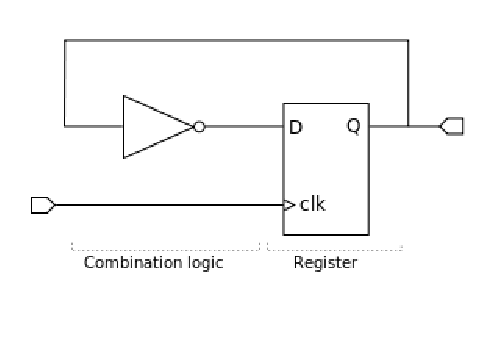
\includegraphics[scale=0.8]{rtl_example.eps}
\end{center}
\caption{Légende}
\label{Référence}
\end{figure}
Le schéma ci-dessus montre comment est représenté un circuit. Nous constatons qu'il est ici totalement fait abstraction de la manière avec laquelle ce dernier est câblé. Nous ne connaissons que ce qui entre et ce qui sort de ce dernier. Un HDL décrira, quant à lui, le {\og}comportement{\fg} externe, générale du circuit.

La principale différence entre les HDL avec les langages de programmations traditionnels est qu'avec un HDL, contrairement aux autres types de langages procéduraux, nous pouvons modéliser de multiples processus parallèles et exprimer le temps de manière explicite. En effet, ces deux éléments (le parallélisme et le temps) sont les principaux attributs d'un matériel électronique. Un changement dans un des processus pourra donc déclencher une mise à jour dans les autres processus.

\subsection{Les autres HDL existants}
Il existe de nombreux HDL autre que les deux plus connu que sont Verilog et VHDL, tel que, Altera HDL (AHDL) qui est un langage propriétaire d'\textbf{Altera}, Hydra qui est basé sur \textbf{Haskell}, MyHDL qui est basé sur \textbf{Python} ou encore RHDL basé sur \textbf{Ruby}. Un autre HDL est SystemC, qui est, avec Verilog et VHDL, un des HDL les plus utilisés dans l'industrie. Cependant, ce dernier n'est pas un langage à part entière puisque c'est en fait un ensemble de classes \textbf{C++} fournissant les outils nécessaires à la modélisation du matériel. De part cette caractéristique, nous ne nous y attarderons pas plus. Milkymist, ceux qui font le SoC sur lequel nous allons travailler, possède aussi leur propre langage Migen qui est toujours en développement, nous y reviendrons dans une sous-section ultérieure.

\subsection{Verilog VS VHDL}
\vspace{15px}
Nous allons vous présenter plus en détail les deux principaux HDL que sont VHDL et Verilog. Chacun à ses atouts :
\begin{itemize}
\item VHDL :
\begin{itemize}
\item ce langage a été fait pour aider la conception et la spécification au niveau d'un système électronique,
\item il est plus souple que Verilog car permet, entre autre, à l'utilisateur de définir ses types, ses configurations, etc.
\end{itemize}
\item Verilog :
\begin{itemize}
\item conçut de base pour les concepteurs de matériel numérique développant des FPGAs et ASICs
\item parfait pour convertir des types de données de vecteurs de bits vers des notations arithmétiques,
\item existence de supports compréhensible pour la conception numérique de bas niveau.
\end{itemize}
\end{itemize}

{Gateway Design Automation Inc.}  puis rendu disponible au grand public en 1990 par \textbf{Cadence}.
Ce sont-là les principales différences entre les deux langages. Dans les faits, VHDL et Verilog sont similaires puisqu'ils sont tous les deux des standards IEEE : \textit{IEEE standard 1076-1987} 
%% FLS: ref bibliographique
en 1987 puis \textit{IEEE standard 1076-1993}
%% FLS: ref bibliographique
 en 1993 après une mise à jour pour VHDL. Il a ensuite été mis à jour régulièrement pour arriver, en 2008 au standard \textit{IEEE 1076}
%% FLS: ref bibliographique
 (VHDL 4.0) qui est la dernière version en date. Verilog est lui devenu un standard en 1995 : \textit{IEEE standard 1364-1995} 
%% FLS: ref bibliographique
et a été mis à jour deux fois depuis : en 2001  \textit{IEEE Standard 1364-2001} 
%% FLS: ref bibliographique
(Verilog 2001) qui corrigera de nombreux problèmes puis en 2005  \textit{IEEE Standard 1364-2005}
%% FLS: ref bibliographique 
(Verilog 2005) qui corrigea quelques bogues. Historiquement, VHDL a été développé pour l'armée de l'air des Etats-Unis d'Amérique (contrat \textit{F33615-83-C-1003}) par \textit{Intermetrics, Inc.}, \textit{Texas Instruments} et \textit{IBM}. \textit{Intermetrics, Inc.}  fournissait les experts en langage (de programmation) et était aussi le maître d'\oe{}uvre du projet. \textit{Texas Instruments} se concentrait sur la partie expertise en conception de puces (électronique). \textit{IBM} quant à lui fournissait les experts en conception de systèmes informatiques. C'était donc un projet d'une certaine envergure (comme \textit{ADA} par exemple). Verilog a quant à lui était lancé en 1984 par \textbf{Gateway Design Automation Inc.}  puis rendu disponible au grand public en 1990 par \textbf{Cadence}.

\subsection{Le HDL de Milkymist : Migen}
Nous vous avions aussi parlé de Migen, le langage de Milkymist. Nous n'allons pas l'utiliser mais il nous semblait intéressant d'en parler. En effet, dans le futur, le SoC Mylkymist utilisera ce langage. Le projet Migen (pour \textbf{Mi}lkymist \textbf{gen}erator) a été lancé en 2011 et est toujours en cours de de développement. Cet outil est basé sur le langage \textbf{Python} et il a pour but d'automatiser encore plus le processus de conception des VSLI (Very-large-scale integration, c'est un processus de création de circuits intégrés). Grâce à Migen, il sera possible d'appliquer des concepts modernes, tel que l'objet et la métaprogramation \footnote{La métaprogrammation c'est la création de programmes qui utilisent d'autres programmes pour fonctionner. Ces autres programmes sont donc les données manipulés par le métaprogramme créé.}  par exemple, pour concevoir un matériel. L'avantage étant que ce qui en résulte est plus élégant et est surtout plus facile à faire évoluer, tout en réduisant les problèmes dûs aux erreurs humaines. Ce sont-là les grands principes que Milkymist veut mettre en place dans Migen. En se basant sur ces dernières, Migen fournira les outils nécessaires pour construire des conceptions synchrones de manière plus productive en automatisant certaines tâches comme réinitialiser les registres et en faisant abstraction du paradigm des HDL basé sur l'évènement (le parallélisme). Migen permettra aussi d'intégrer le SoC (\textit{system-on-chip}) en automatisant par exemple l'interconnexion entre les chips (puces). Migen accélérera aussi la conception matériel grâce le paradigme du flux de données avec une intégration semi automatique dans le SoC.
 
Migen semble donc un projet très intéressant puisqu'il rend la conception plus simple et qu'il rend plus efficace le matériel. Cependant, ce projet est encore jeune et encore en développement, toutes les fonctionnalités ne sont pas encore implémentées. Nous ne l'utiliserons donc pas dans notre projet pour éviter tout problème.
